% Standalone 10-minute review. Not part of 2026-10-28-Meeting-Main.tex.
% Page numbers are 1/N of this deck only.
% Compile with pdfLaTeX from this directory.
\documentclass[aspectratio=169,10pt]{beamer}
\usepackage[english]{babel}
\usepackage[utf8]{inputenc}
\usepackage[T1]{fontenc}
\usepackage{lmodern}
\usepackage{amsmath,amssymb}
\usepackage{booktabs,tabularx,array}
\usepackage{graphicx}
\graphicspath{{./}{figures/}}
\usepackage{xcolor}
\usepackage{tikz}
\usetikzlibrary{arrows.meta,positioning,calc,shapes.geometric}
\usepackage{hyperref}

\usetheme{Madrid}
\usecolortheme{default}
\definecolor{Ink}{HTML}{243748}
\definecolor{Muted}{HTML}{667B8B}
\definecolor{Accent}{HTML}{347E74}
\definecolor{AccentBlue}{HTML}{507DAD}
\definecolor{SoftMint}{HTML}{E6F4EE}
\definecolor{SoftBlue}{HTML}{E9F2F9}
\definecolor{SoftLilac}{HTML}{F1EEF8}
\definecolor{Paper}{HTML}{FBFCFE}
\definecolor{Divider}{HTML}{D8E4EB}

\setbeamercolor{background canvas}{bg=Paper}
\setbeamercolor{normal text}{fg=Ink}
\setbeamercolor{structure}{fg=Accent}
\setbeamercolor{frametitle}{fg=Ink,bg=SoftBlue}
\setbeamercolor{title}{fg=Ink}
\setbeamercolor{subtitle}{fg=Muted}
\setbeamercolor{block title}{fg=Ink,bg=SoftBlue}
\setbeamercolor{block body}{fg=Ink,bg=white}
\setbeamercolor{item}{fg=Accent}
\setbeamercolor{caption name}{fg=Muted}
\setbeamercolor{footline}{fg=Muted,bg=Paper}
\setbeamerfont{frametitle}{size=\large,series=\bfseries}
\setbeamerfont{footline}{size=\tiny}
\setbeamerfont{block title}{series=\bfseries}
\setbeamertemplate{headline}{}
\setbeamertemplate{navigation symbols}{}
\setbeamertemplate{blocks}[rounded][shadow=false]
\setbeamertemplate{itemize items}[circle]
\setbeamertemplate{itemize subitem}[circle]
\setbeamertemplate{footline}{%
  \leavevmode\hbox{%
    \begin{beamercolorbox}[wd=\paperwidth,ht=.30cm,dp=.16cm,rightskip=.60cm plus 1fil]{footline}%
      \hfill\insertframenumber\,/\,\inserttotalframenumber
    \end{beamercolorbox}}}
\setbeamertemplate{frametitle}{%
  \nointerlineskip
  \begin{beamercolorbox}[wd=\paperwidth,ht=.72cm,dp=.16cm,leftskip=.55cm,rightskip=.40cm]{frametitle}%
    \usebeamerfont{frametitle}\insertframetitle
  \end{beamercolorbox}}

\newcommand{\smalllabel}[1]{{\scriptsize\bfseries\color{Accent}\MakeUppercase{#1}}}
\newcommand{\hint}[1]{{\footnotesize\color{Muted}#1}}
\newcommand{\takeaway}[1]{%
  \begin{beamercolorbox}[rounded=true,sep=0.16cm,wd=\linewidth]{block title}%
    {\normalsize\bfseries #1}
  \end{beamercolorbox}}
\newcommand{\stepcard}[3]{%
  \begin{beamercolorbox}[rounded=true,sep=0.16cm,wd=\linewidth]{block body}%
    {\footnotesize\bfseries\color{Accent}#1}\par\vspace{1.1mm}
    {\large\bfseries #2}\par\vspace{1.1mm}
    {\footnotesize\color{Muted}#3}%
  \end{beamercolorbox}}

\newcommand{\figureplaceholder}[3]{%
  \begingroup\centering
  \IfFileExists{#1}{%
    \includegraphics[width=.98\linewidth,height=#2,keepaspectratio]{#1}%
  }{%
    \IfFileExists{figures/#1}{%
      \includegraphics[width=.98\linewidth,height=#2,keepaspectratio]{figures/#1}%
    }{%
      \begin{tikzpicture}
        \node[draw=AccentBlue!55,dashed,line width=.7pt,rounded corners=4pt,
              fill=SoftBlue!60,minimum height=#2,minimum width=.95\linewidth,
              text width=.85\linewidth,align=center,inner sep=2mm] {
           {\color{AccentBlue}\bfseries FIGURE PLACEHOLDER}\\[2.2mm]
           {\color{Ink}\small #3}\\[1.5mm]
           {\color{Muted}\scriptsize\ttfamily\detokenize{#1}}};
      \end{tikzpicture}%
    }%
  }\par\endgroup}

\newcommand{\src}[1]{\vspace{0.12cm}\hint{Source: #1}}


\newcommand{\mainfig}[2]{%
  \begingroup\centering
  \includegraphics[width=\linewidth,height=#2,keepaspectratio]{#1}\par
  \endgroup}

\title{10-minute Paper Review: ThunderServe and Hetis}
\author{Yu-Jui Liang}
\date{28 Oct 2026}
\subject{10-minute paper review, 28 Oct 2026}
\begin{document}
\begin{frame}
\vspace{.22cm}
{\large\bfseries\color{Accent}10-MINUTE PAPER REVIEW\par}\vspace{.26cm}
{\LARGE\bfseries Heterogeneous Model Serving\\[.16cm]at Different Granularities\par}
\vspace{.20cm}{\LARGE\color{Muted}ThunderServe and Hetis\par}
\vspace{.26cm}{\Large\textbf{Yu-Jui Liang}\par}
\vspace{.10cm}{\large Advisor: Hsiang-Yun Cheng\par}
\vspace{.08cm}{\large National Taiwan University \quad | \quad Academia Sinica\par}
\vspace{.08cm}{\large 28 Oct 2026\par}
\vfill
{\footnotesize\color{Muted}ThunderServe: Youhe Jiang et al., MLSys 2025\\
Hetis: Zizhao Mo et al., SC 2025}\par
\vspace{.08cm}{\color{Accent}\rule{\textwidth}{.7pt}}
\end{frame}

\begin{frame}{Presentation Roadmap}
  \smalllabel{28 Oct / Plan}\par
  \vspace{.38cm}
  \begin{enumerate}
    \setlength{\itemsep}{.48cm}
    \item \textbf{\large ThunderServe + Hetis}\par
      {\normalsize\color{Muted}10 minutes. Review and comparison of last week's papers. This deck.}
    \item \textbf{\large Helix}\par
      {\normalsize\color{Muted}10 minutes. Concise report on a new paper.}
    \item \textbf{\large Tessera}\par
      {\normalsize\color{Muted}10 minutes. Concise report on a new paper.}
    \item \textbf{\large Two HBF papers}\par
      {\normalsize\color{Muted}Extra 10 minutes. Backup, not counted in the formal 30 minutes.}
  \end{enumerate}
  \vspace{.36cm}\hint{Formal report: three blocks, 30 minutes. This deck is the first block.}
\end{frame}

% ThunderServe 4-minute summary. Input from 2026-10-28-Meeting-Main.tex.
% Figures are copies of 2026-10-21-meeting/ThunderServe/. See SOURCE.txt.
% Facts checked against 2026-10-21-meeting/MLSys25_Thunderserve.pdf.

\begin{frame}[t]{Why Heterogeneous GPU Serving Needs Phase-Aware Scheduling}
\begin{columns}[T,onlytextwidth]
\begin{column}{.50\textwidth}
\mainfig{ThunderServe/ThunderServe_Fig01.png}{3.85cm}
\end{column}
\begin{column}{.48\textwidth}
{\footnotesize\textbf{Observation}}
\begin{itemize}\setlength{\itemsep}{.04cm}\footnotesize
\item Prefill: compute-intensive.
\item Decode: memory-bandwidth-intensive.
\end{itemize}
\vspace{.06cm}
{\scriptsize A40: 149.7 FP16 TFLOPS. 3090 Ti: 1008 GB/s. Table~1.}
\vspace{.12cm}
{\footnotesize\textbf{Challenge}}
\begin{itemize}\setlength{\itemsep}{.04cm}\footnotesize
\item Heterogeneous GPU resources.
\item Limited and heterogeneous network bandwidth.
\item KV cache transfer overhead.
\end{itemize}
\vspace{.08cm}
{\footnotesize\textbf{Research question}\par}
{\footnotesize How to jointly optimize GPU allocation, phase placement, and communication?\par}
\end{column}
\end{columns}
\vspace{.08cm}
\takeaway{The better GPU can differ by phase. KV transfer makes a FLOPS-only or bandwidth-only split insufficient.}
\src{ThunderServe Sec.~1, Fig.~1, Table~1. Prices in the figure are per request.}
\end{frame}

\begin{frame}[t]{Joint Optimization of GPU Placement, Parallelism, and Routing}
\begin{columns}[T,onlytextwidth]
\begin{column}{.60\textwidth}
\mainfig{ThunderServe/ThunderServe_Fig03.png}{4.70cm}
\end{column}
\begin{column}{.38\textwidth}
\smalllabel{Upper-level --- Tabu search}\par
\begin{itemize}\setlength{\itemsep}{.04cm}\footnotesize
\item GPU group construction.
\item Prefill / decode phase designation.
\end{itemize}
\vspace{.08cm}
\smalllabel{Lower-level --- configuration}\par
\begin{itemize}\setlength{\itemsep}{.04cm}\footnotesize
\item TP / PP configuration.
\item Prefill / decode request routing.
\item Network-aware KV cache transfer.
\end{itemize}
\vspace{.08cm}
{\scriptsize Additional mechanisms: KV cache compression and lightweight rescheduling.}
\end{column}
\end{columns}
\vspace{.04cm}
\takeaway{Upper level assigns groups and phases. Lower level sets parallelism and routing. Together they score one deployment plan.}
\src{ThunderServe Sec.~3.2--3.4, Fig.~3.}
\end{frame}

\begin{frame}[t]{Does Phase-Aware Scheduling Improve Serving Efficiency?}
{\scriptsize\textbf{Question:} Does workload-aware phase placement raise end-to-end throughput?\par}
\vspace{.06cm}
\begin{columns}[T,onlytextwidth]
\begin{column}{.46\textwidth}
\smalllabel{Experiment 1 --- Table 3}\par
{\footnotesize\textbf{Workload-aware deployment}\par}
\vspace{.04cm}
{\footnotesize Coding: \textbf{8 prefill / 4 decode}\par}
{\footnotesize Conversation: \textbf{4 prefill / 8 decode}\par}
\vspace{.06cm}
{\scriptsize LLaMA-30B, same 32-GPU cloud pool. Coding has longer prompts; conversation has longer outputs.\par}
\vspace{.10cm}
\smalllabel{Experiment 2 --- Figure 9}\par
\vspace{.04cm}
{\scriptsize\renewcommand{\arraystretch}{1.08}
\begin{tabular}{@{}lcc@{}}\toprule
 & \textbf{Coding} & \textbf{Conv.}\\\midrule
vs.\ HexGen & $1.5\times$ & $1.3\times$\\
vs.\ DistServe & $1.5\times$ & $2.1\times$\\\bottomrule
\end{tabular}\par}
\vspace{.05cm}
{\scriptsize HexGen: heterogeneous cloud GPUs.\par
DistServe: homogeneous 8$\times$A100, similar price. Not the same machines.\par}
\end{column}
\begin{column}{.52\textwidth}
\mainfig{ThunderServe/ThunderServe_Fig09.png}{3.35cm}
\vspace{.06cm}
{\scriptsize vLLM, the fourth group, is also in-house. HexGen and DistServe are different hardware setups.\par}
\end{column}
\end{columns}
\vspace{.08cm}
\takeaway{Workload-aware placement improves overall serving throughput under heterogeneous resource constraints.}
\src{ThunderServe Sec.~5.1--5.3, Fig.~9, Table~3. Relative throughput is ThunderServe over each baseline.}
\end{frame}

\begin{frame}[t]{Phase-Aware Deployment Improves Cost Efficiency}
\vspace{.08cm}
\begin{columns}[T,onlytextwidth]
\begin{column}{.32\textwidth}
\stepcard{1. JOINT OPTIMIZATION}{One deployment plan}{GPU grouping, phase designation, TP/PP, and request routing.}
\end{column}
\begin{column}{.32\textwidth}
\stepcard{2. PERFORMANCE}{1.7$\times$ average, up to 2.1$\times$}{Overall throughput claim in the paper. Not one bar of Figure~9.}
\end{column}
\begin{column}{.32\textwidth}
\stepcard{3. DYNAMIC ADAPTATION}{Full 157 s, lightweight 13 s}{Table~4 overall time. The gap includes model reload, not search time alone.}
\end{column}
\end{columns}
\vspace{.16cm}
{\scriptsize Table~4 breakdown. Full: rescheduling 54($\pm$5)\,s $+$ reload 103($\pm$10)\,s $=$ 157($\pm$13)\,s.
Lightweight: rescheduling 13($\pm$2)\,s $+$ reload 0\,s $=$ 13($\pm$2)\,s.\par}
\vspace{.12cm}
\takeaway{ThunderServe demonstrates that heterogeneous GPU serving benefits from jointly optimizing inference phases, hardware allocation, and communication.}
\vspace{.08cm}
{\footnotesize ThunderServe focuses on phase-level resource allocation; finer-grained workload partitioning is another possible direction.\par}
\src{Abstract and Sec.~6 for the 1.7$\times$/2.1$\times$ claim. Sec.~5.4 and Table~4 for rescheduling time.}
\end{frame}

% Hetis 4-minute summary. Input from 2026-10-28-Meeting-Main.tex.
% Figures are copies of 2026-10-21-meeting/Hetis/. See SOURCE.txt.
% Facts checked against 2026-10-21-meeting/SC25_Hetis.pdf.

\begin{frame}[t,label=main_hetis_why]{Hetis: Why Static Parallelism Wastes GPU Resources}
\begin{columns}[T,onlytextwidth]
\begin{column}{.56\textwidth}
\mainfig{Hetis/Hetis_Fig02.png}{4.55cm}
\end{column}
\begin{column}{.42\textwidth}
{\normalsize\textbf{Why one parallelism for every module?}}
\begin{itemize}\setlength{\itemsep}{.12cm}\footnotesize
\item \qlink{backup_hetis_motivation_01}{MLP} and decode \qlink{backup_hetis_motivation_01}{attention} do not show the same GPU gap.
\item A low-end GPU can drag dense computation.
\item A static split can also leave \qlink{backup_hetis_motivation_01}{KV-cache} space idle.
\end{itemize}
\vspace{.14cm}
{\footnotesize Fig.~2 is one Llama-70B decode layer, sequence length 1000. Not end-to-end latency, and not a bandwidth chart.}
\vspace{.12cm}
{\footnotesize The paper asks for module-aware, fine-grained, dynamic parallelism.}
\end{column}
\end{columns}
\vspace{.14cm}
\takeaway{GPU performance heterogeneity is module-dependent; static model partitioning cannot efficiently balance both computation and memory.}
\src{Hetis Sec.~2.2--2.4, Figs.~1--2. Text: P100 lags A100 by up to $40.4\times$ on average in decode MLP.}
\end{frame}

\begin{frame}[t,label=main_hetis_arch]{Hetis: Selective Primary Workers and Dynamic Head-wise Attention}
\begin{columns}[T,onlytextwidth]
\begin{column}{.46\textwidth}
\mainfig{Hetis/Hetis_Fig03.png}{4.55cm}
\end{column}
\begin{column}{.52\textwidth}
{\footnotesize
\textbf{\qlink{backup_hetis_workers_01}{PRIMARY WORKERS}}\par
Parallelizer searches dense-compute plus communication cost. They jointly hold the model with TP/PP, and DP when needed. They run prefill, decode dense modules, and heads that stay local.\par
\vspace{.01cm}
\textbf{\qlink{backup_hetis_workers_01}{ATTENTION WORKERS}}\par
GPUs that add little to dense compute. They run some decode attention and its KV cache, without a second full copy of the weights. Default exclusion threshold $\Delta=0.05$. Selection is cost, not a FLOPS or bandwidth ranking.\par
\vspace{.01cm}
\textbf{\qlink{backup_hetis_headwise_01}{PER-LAYER DECODE TRAFFIC}}\par
Primary computes QKV. For an offloaded head it sends that token's Q/K/V; the worker attends with its stored KV cache and returns the output. Full history is not resent each step. GQA keeps a query group with its KV heads.\par}
\end{column}
\end{columns}
\vspace{.00cm}
\takeaway{Hetis concentrates dense computation on suitable GPUs while dynamically distributing decode attention at \qlink{backup_hetis_headwise_01}{head granularity}.}
\src{Hetis Sec.~3--5, Fig.~3. Fig.~3 also names Profiler, Dispatcher, and Hauler.}
\end{frame}

\begin{frame}[t,label=main_hetis_results]{Hetis: Does Head-wise Parallelism Improve Serving Performance?}
{\footnotesize\textbf{Setup:} 4$\times$A100-80GB, 4$\times$3090, 4$\times$P100 on four hosts, 100\,Gbps between hosts. Llama-13B, OPT-30B, Llama-70B. Baselines: Splitwise, Hexgen. Workloads: ShareGPT, HumanEval, LongBench.}
\begin{columns}[T,onlytextwidth]
\begin{column}{.60\textwidth}
\smalllabel{Q1 --- end-to-end serving}\par
{\footnotesize Fig.~10 y-axis is latency (s/token), not throughput.\par}
\vspace{.02cm}
\mainfig{Hetis/Hetis_Fig10.png}{2.70cm}
\end{column}
\begin{column}{.38\textwidth}
{\footnotesize Up to $2.25\times$ \qlink{backup_hetis_results_01}{throughput} vs.\ Splitwise, and $1.33\times$ vs.\ Hexgen. Maxima across settings, not averages.}
\vspace{.02cm}
{\footnotesize On this \qlink{backup_hetis_results_01}{Llama-70B} run, A100 and 3090 were primaries and P100s were attention workers. A search result, not a ranking.}
\vspace{.02cm}
\smalllabel{Q2 --- KV cache}\par
\mainfig{Hetis/Hetis_Fig11.png}{1.75cm}
{\footnotesize Up to $1.87\times$ available \qlink{backup_hetis_results_01}{KV cache} versus the tested baselines.}
\end{column}
\end{columns}
\takeaway{Fine-grained attention placement improves serving capacity by reducing compute imbalance and KV cache underutilization.}
\src{Hetis Sec.~7.1--7.3, Figs.~8--13. The $1.49\times$ figure is decode-attention module latency, not end-to-end latency.}
\end{frame}

\begin{frame}[t,label=main_hetis_close]{Hetis: Main Contributions and Takeaways}
\vspace{.10cm}
\begin{columns}[T,onlytextwidth]
\begin{column}{.32\textwidth}
\stepcard{1}{Module-aware workers}{Assign GPUs by what each module costs, not by one static split of the whole model.}
\end{column}
\begin{column}{.32\textwidth}
\stepcard{2}{Head-level attention}{Offload decode attention by heads. Unselected heads stay on the primary.}
\end{column}
\begin{column}{.32\textwidth}
\stepcard{3}{\qlink{backup_hetis_migration_01}{Online adaptation}}{\qlink{backup_hetis_migration_01}{Dispatcher} reallocates heads. \qlink{backup_hetis_migration_01}{Hauler} migrates \qlink{backup_hetis_migration_01}{KV cache} at head granularity.}
\end{column}
\end{columns}
\vspace{.28cm}
{\normalsize\textbf{Implementation: vLLM extension.}\par}
\vspace{.08cm}
{\footnotesize Head-level KV-cache blocks, custom CUDA kernels, NCCL peer-to-peer, and reuse of PagedAttention. Base framework, not a Hetis repository: \url{https://github.com/vllm-project/vllm}\par}
\vspace{.12cm}
{\footnotesize End-to-end results use the real GPU cluster. Sec.~7.4 adds a large-scale simulation of parallelizer search cost.\par}
\vspace{.18cm}
\takeaway{Hetis improves heterogeneous GPU utilization through module-aware, fine-grained, and dynamic parallelism.}
\src{Hetis Sec.~6 and Sec.~9 for the system; Sec.~7.1--7.2 for the cluster results; Sec.~7.4 for the search simulation.}
\end{frame}

% One comparison frame. The diagrams are conceptual, not paper figures.
% Facts checked against the local ThunderServe and Hetis PDFs.

\begin{frame}[t,label=main_compare]{ThunderServe vs.\ Hetis: Different Granularities of GPU Specialization}
\vspace{.02cm}
\begin{columns}[T,onlytextwidth]
\begin{column}{.48\textwidth}
{\centering
{\footnotesize\bfseries ThunderServe}\\[1.5mm]
\begin{tikzpicture}[
  every node/.style={font=\footnotesize, align=center, inner sep=2.5pt},
  box/.style={draw=Accent, rounded corners=2pt, fill=SoftMint, minimum height=9mm, text width=20mm}
]
\node[box] (pre) {Prefill\\group};
\node[box, right=9mm of pre] (dec) {Decode\\group};
\draw[-{Stealth}, thick, Accent] (pre) -- node[above, font=\footnotesize, text=Ink] {\qlink{backup_ts_kv_01}{KV cache}} (dec);
\end{tikzpicture}\\[1.5mm]
{\footnotesize deployment-level groups\par}}
\end{column}
\begin{column}{.48\textwidth}
{\centering
{\footnotesize\bfseries Hetis}\\[1.5mm]
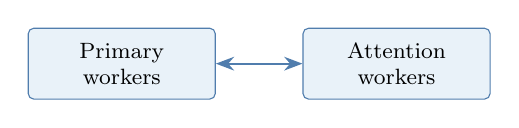
\begin{tikzpicture}[
  every node/.style={font=\footnotesize, align=center, inner sep=2.5pt},
  box/.style={draw=AccentBlue, rounded corners=2pt, fill=SoftBlue, minimum height=9mm, text width=22mm}
]
\node[box] (pri) {Primary\\workers};
\node[box, right=11mm of pri] (att) {Attention\\workers};
\draw[{Stealth}-{Stealth}, thick, AccentBlue] (pri) -- (att);
\end{tikzpicture}\\[1.5mm]
{\footnotesize head-level decode attention\par}}
\end{column}
\end{columns}
\vspace{.06cm}
{\scriptsize\renewcommand{\arraystretch}{1.12}
\begin{tabularx}{\textwidth}{@{}>{\bfseries}p{2.15cm}>{\raggedright\arraybackslash}X>{\raggedright\arraybackslash}X@{}}
\toprule
 & \textbf{ThunderServe} & \textbf{Hetis}\\\midrule
Objective & Cost-efficient serving under workload and network limits & Less compute imbalance and better \qlink{backup_hetis_results_01}{memory use}\\
Granularity & Prefill / decode phases & Dense modules / attention heads\\
Weights & Each phase replica hosts weights; TP/PP allowed & Primaries hold the model. Attention workers do not\\
Communication & KV cache between prefill and decode replicas & Current-token Q/K/V and outputs for offloaded heads\\
Scheduling & Grouping, phase, TP/PP, routing, lightweight rescheduling & Primary selection, online head dispatch, KV migration\\\bottomrule
\end{tabularx}\par}
\vspace{.06cm}
\takeaway{ThunderServe optimizes \qlink{backup_ts_phase_01}{phase-level} deployment; Hetis optimizes module-aware execution and \qlink{backup_hetis_headwise_01}{head-level} attention placement.}
\src{Diagrams are conceptual, not paper figures. Do not rank the papers by peak throughput: hardware, workloads, and baselines differ.}
\end{frame}


\begin{frame}
\vfill
\begin{center}
{\large\bfseries\color{Accent}10-MINUTE PAPER REVIEW\par}
\vspace{.72cm}
{\fontsize{34}{40}\selectfont\bfseries Thank you\par}
\vspace{.42cm}
{\LARGE\color{Muted}ThunderServe and Hetis\par}
\vspace{.62cm}
{\Large\textbf{Yu-Jui Liang}\par}
\vspace{.18cm}
{\Large\color{Muted}28 Oct 2026\par}
\end{center}
\vfill
\end{frame}
\end{document}
